%FILL THESE IN
\def\mytitle{Solar System Model}
\def\mykeywords{Fill, These, In, So, google, can, find, your, report}
\def\myauthor{Dimitrios Tsolis}
\def\contact{40204497@live.napier.ac.uk}
\def\mymodule{Module Title (SET08116)}
%YOU DON'T NEED TO TOUCH ANYTHING BELOW
\documentclass[10pt, a4paper]{article}
\usepackage[a4paper,outer=1.5cm,inner=1.5cm,top=1.75cm,bottom=1.5cm]{geometry}
\twocolumn
\usepackage{graphicx}
\graphicspath{{./images/}}
%colour our links, remove weird boxes
\usepackage[colorlinks,linkcolor={black},citecolor={blue!80!black},urlcolor={blue!80!black}]{hyperref}
%Stop indentation on new paragraphs
\usepackage[parfill]{parskip}
%% all this is for Arial
\usepackage[english]{babel}
\usepackage[T1]{fontenc}
\usepackage{uarial}
\renewcommand{\familydefault}{\sfdefault}
%Napier logo top right
\usepackage{watermark}
%Lorem Ipusm dolor please don't leave any in you final repot ;)
\usepackage{lipsum}
\usepackage{xcolor}
\usepackage{listings}
%give us the Capital H that we all know and love
\usepackage{float}
%tone down the linespacing after section titles
\usepackage{titlesec}
%Cool maths printing
\usepackage{amsmath}
%PseudoCode
\usepackage{algorithm2e}
%urlreference
\usepackage{url}



\titlespacing{\subsection}{0pt}{\parskip}{-3pt}
\titlespacing{\subsubsection}{0pt}{\parskip}{-\parskip}
\titlespacing{\paragraph}{0pt}{\parskip}{\parskip}
\newcommand{\figuremacro}[5]{
    \begin{figure}[#1]
        \centering
        \includegraphics[width=#5\columnwidth]{#2}
        \caption[#3]{\textbf{#3}#4}
        \label{fig:#2}
    \end{figure}
}

\lstset{
	escapeinside={/*@}{@*/}, language=C++,
	basicstyle=\fontsize{8.5}{12}\selectfont,
	numbers=left,numbersep=2pt,xleftmargin=2pt,frame=tb,
    columns=fullflexible,showstringspaces=false,tabsize=4,
    keepspaces=true,showtabs=false,showspaces=false,
    backgroundcolor=\color{white}, morekeywords={inline,public,
    class,private,protected,struct},captionpos=t,lineskip=-0.4em,
	aboveskip=10pt, extendedchars=true, breaklines=true,
	prebreak = \raisebox{0ex}[0ex][0ex]{\ensuremath{\hookleftarrow}},
	keywordstyle=\color[rgb]{0,0,1},
	commentstyle=\color[rgb]{0.133,0.545,0.133},
	stringstyle=\color[rgb]{0.627,0.126,0.941}
}

\thiswatermark{\centering \put(336.5,-38.0){\includegraphics[scale=0.8]{logo}} }
\title{\mytitle}
\author{\myauthor\hspace{1em}\\\contact\\Edinburgh Napier University\hspace{0.5em}-\hspace{0.5em}\mymodule}
\date{}
\hypersetup{pdfauthor=\myauthor,pdftitle=\mytitle,pdfkeywords=\mykeywords}
\sloppy



\begin{document}
	
		\hyphenchar\font=-1    
	
	\maketitle
	\begin{abstract}
	The aim of this project was to render a realistic scene using the skills developed in the Computer Graphics Module at Edinburgh Napier University using OpenGL and C++. The scene produced in this project is a solar system, inspired by my adoration for the stars and the Star Wars movies \cite{StarWars}. I was also inspired by some of the previous Computer Graphics Projects \cite{PreviousProjects}. Additionally, I gained inspiration from a Youtube tutorial\cite{Tutorial} for the bloom effect. Advanced 3D effects and techniques are used to accomplish the generated result, such as lighting,shadowing and texturing. These techniques are widely used in a variety of games.
	\figuremacro{h}{MillenniumFalcon}{Millenium Falcon}{ - Chase Camera Inspiration}{1.0}
	\end{abstract}
    
	\textbf{Keywords -- }{Shadowing, Lighting, Multi-Texturing, Skybox, Multiple Cameras, Material Shading}
    %START FROM HERE
	\section{Introduction}
    \paragraph{Referencing}

    The key effects being used are lighting, texturing, shadowing, skybox, material shading and transformation hierarchy. Various rendering techniques are required to produce a realistic depiction of the scene. The different lights being used in the scene are a spot light and a point light in the middle of the sun. Transformation techniques are also being applied to the different meshes of the scene, and each of the objects render have their own textures.Furthermore, in order to create the stars image around the solar system a skybox effect is being used. In order to make the earth more realistic, normal mapping is being implemented on the project.
    
    Diffuse light is being applied to the scene, adding some depth perception to the objects, as well as specular light which adds shininess of materials to objects and changes depending on the camera position. The transformation and translating of the meshes in the scene is the scaling and the positioning of the objects. Texturing combined with the lighting is applied to give the objects a more realistic aesthetic.  A more advanced technique being used is normal mapping, which uses the texture and a normal mapped version of the texture, which helps determines the direction the pixels are facing, giving an extra feeling of depth to the object. Finally, some advanced post-rendering techniques have been added, like motion blur, bloom and lens flare.
    
    
	
	\section{Related Work}
	\iffalse
	\paragraph{Formatting}
	Some common formatting you may need uses these commands for \textbf{Bold Text}, \textit{Italics}, and \underline{underlined}.
	\fi
	
	The implementations required for this project have been based on the Computer Graphics workbook \cite{Workbook}, while some of the skills attained had to be further developed. For example, I learned how to apply textures from the workbook, but I also learned how to apply multiple textures and normal mapping by creating texture arrays and binding them to the corresponding meshes in the render boolean by looking up information on-line and experimenting with OpenGl.
	
	\iffalse
	
	\subsection{LineBreaks}
	Here is a line
    
    Here is a line followed by a double line break.
	This line is only one line break down from the above, Notice that latex can ignore this
    
    We can force a break \\ with the break operator.
	
	\subsection{Code Listing}
    You can load segments of code from a file, or embed them directly.
    
\begin{lstlisting}[caption = Hello World! in c++]
#include <iostream>

int main() {
    std::cout << "Hello World!" << std::endl;
    std::cin.get();
    return 0;
}
\end{lstlisting}

\lstinputlisting[caption = Hello World! in python script]{./sourceCode/hello.py}

	\fi
	
	

	
	
\section{Implementation}
	A variety of visual elements were involved in the creation of the scene. These elements are:
	\begin{itemize}
		\item Texturing
		\item Normal Mapping
		\item Lighting
		\item Shadow Mapping
		\item Transform Hierarchy
		\item Skybox
		\item Particles Effect
		\item Motion Blur
		\item Bloom Effect
		\item Lens Flare Effect
	\end{itemize}
	Apart from these visual elements, multiple cameras and the rotation of the planets around the sun were also implemented.
%\newpage
\subsection{Texturing}

	\figuremacro{H}{Jupiter}{Jupiter Texture}{ - Texture Example}{1.0}

	In this project I have created a mesh array and a texture array. In order to apply a texture to a specific mesh, the same name is given to the mesh and the texture in their corresponding arrays. So during the render method, I have created a for loop to render each mesh, and each time a mesh is rendered by going through the for loop, the texture is bound to the mesh by checking for a texture with the exact same name. During the for loop, the key element of the mesh array is the same in the texture array, and therefore, the texture is bound. An example of a texture can bee seen in figure \textbf{\ref{fig:Jupiter}}.


\subsection{Normal Mapping}
		
	\figuremacro{H}{Earth}{Normal Mapped Earth}{ }{1.0}
	
	Normal mapping is a method used for making fake bumps and dents in the object, basically to make it more realistic. This is achieved by calculating the normals on a per pixel basis instead of per vertex basis. A normal map is basically a texture  where the x, y and z axis of the normals are represented by red, green and blue values respectively. In order for normal mapping to be used, we need to work within the tangent coordinate space, which is based on the normal at a particular point of the object. So when normal mapping is used, the normal, the binormal and the tangent become the axes in our coordinate space. To do this, we simply create a transformation matrix:
	
	    \[
	    TBN=
	    \begin{bmatrix}
	    T_x & B_x & N_x  \\
	    T_y & B_y & N_y  \\
	    T_x & B_x & N_z
	    \end{bmatrix}
	    \]
	    
	where T is the tangent, B is the binormal and N is the normal. These are transformed by the normal matrix in order to get the actual surface values. In our normal mapping shader, we use the TBN matrix to transform the sampled normal. In this project, normal mapping is only applied to the earth (See figure \textbf{\ref{fig:Earth}}).
	
\subsection{Lighting}

	\figuremacro{H}{Moon}{Moon}{ - Emissive light example}{1.0}

	\paragraph{General Lighting} Lighting involves three pieces of physical transformation, which are light emitters, materials and sensors. 
	
	Light sources emit light. A simplistic model of light is considered to have three components:
		\begin{itemize}
			\item \textbf{Ambient Light}: light that shines everywhere at an equal measure
			\item \textbf{Diffuse Light}: light that has a direction and reacts with an object's surface in a different  way depending on the direction of the light
			\item \textbf{Specular Light}: specular highlights
		\end{itemize}
	In this scene, we are not using ambient light, but diffuse and specular, which are calculated in the fragment shaders.
	
	
	Materials describe the surfaces of objects. In our scene, the material description in the shader has three values: emissive colour, diffuse reflection colour, specular reflection colour and shininess. The diffuse reflection colour illustrates how the diffuse and the ambient light interacts with the object, the specular reflection colour describes how the specular light interacts with the object, the shininess describes how shiny the objects looks and the emissive colour is the light that emits from the object. Most of these objects in the scene have those values being set throughout the main cpp file. An example of a material with a relatively high emissive light compared to the other objects is the moon(See figure \textbf{\ref{fig:Moon}}), since most of the planets in this project have their emissive colour set to 0.
	
	Finally, in order for an object to be visible, the light that is interacting with the object has to partially be absorbed by a light sensor. The more light it absorbs, the less visible it is.
	
	
	\figuremacro{H}{Sun}{Point Light}{ - Main Light Source for the project}{1.0}
	
	\paragraph{Point Light}  Point lights are light sources which have a position and an area which they light. In the scene being created, we have one main light source, which is a point light, and it is located in the middle of the sun. In order to let the light go out from inside the sphere, the normals of the sun mesh had to be reversed. I did that by creating a different sun effect which has identical shaders with the normal effect, apart from the vertex shader. In that vertex shader, when the transformed normal is calculated, it is timed by -1, so the normals are reversed and the light can shine throughout the scene.
	
	\figuremacro{H}{Spotlight_Shadow}{Spot Light Example}{ - This is the spotlight that is bound to the shadow map}{1.0}
	
	\paragraph{Spot Lights} Aside from the point light, we have several other spotlights. Spotlights are very similar to point lights, but in this case the lights are facing towards a specific direction. In this coursework, 9 different spotlights are being created. Eight of those spotlights are rotating along along with the planets, with a position over the planets and a direction towards them. The ninth spotlight is under the sun, facing towards the plane and is bound to the shadow map(See figure \textbf{\ref{fig:Spotlight_Shadow}}). Nine different spotlights are being created by using a vector container, which holds the spotlights and their key values. In order for the spotlights to shine, each spotlight should be initialized before rendering. The spotlights in the project can be turned on and off at any time.
	



\subsection{Shadow Mapping}

	\figuremacro{H}{Shadow_Explanation}{Shadow Mapping}{ }{1.0}
	
	In order to implement shadows in this project, we used the shadow mapping technique (See figure \textbf{\ref{fig:Shadow_Explanation}}). Shadow Mapping utilises the depth buffer in order to determine whether an object is in shadow or not. The concept of shadow mapping is that the scene is rendered from the point of view of the light source, then the depth information is gathered, and thereupon that information is used to determine if the object is in shadow. In this scene, I am creating a spot light below the sun facing towards the plane, with a 90 degree point of view, and I am binding the shadow map to that specific light. Therefore, the shadow of the cube is created(See figure \textbf{\ref{fig:Cube_Shadow}}).
	
	
	\figuremacro{H}{Cube_Shadow}{Shadow of the rotating cube}{ }{1.0}
	

\subsection{Transform Hierarchy}

	\figuremacro{H}{Invader}{Space Invader}{ - Transform Hierarchy Implementation}{1.0}
	
	In the scene, transformation hierarchy is applied in one of the objects(See figure \textbf{\ref{fig:Invader}}). During the transformation hierarchy render, the projection matrix(P) and the view matrix(V) are calculated only whenever the camera moves. The model Matrix only changes when a model is moved, rotated, or transformed. When we calculate the model matrix in this case, we set it to be the space invader transform matrix, and then we set it to be the sun transformation matrix(which is rotating around its own y axis) times itself. This makes the space invader object inherit the sun's rotation. The object is located in the middle of the sun.
	
\subsection{Skybox}

	A skybox is implimented in the scene. That gives of the illusion of the stars located around the solar system. In order to to that, a simple cube is rendered, with the inside faces rendered and a star cube map texture applied to it. Furthermore, the depth buffer is temporarily disabled during the skybox render, ensuring that the skybox appears off in the distance. This is achieved by making the position of the skybox equal to the position of the active camera, which means that the camera can never leave the skybox.
	
\subsection{Particles Effect}

	\figuremacro{H}{Explosion}{Explosion}{ - Death Star Explosion using particles and exploding factor}{0.985}
	
	In the scene, a particle simulation is applied, which is one of the simplest form of physics we can have using OpenGL (See figure \textbf{\ref{fig:Explosion}}). A particle is just a physical object that has a velocity and a position. In order to update a particle, the position is changed. In order to implement a more realistic explosion, the velocity is multiplied by a random value so each particle will have different speed. In order to apply the particles effect, Transform Buffers were used. The buffers were created with OpenGL, then the data is set for the buffers, and then the data for the transform feedback is described in the shader. In this particular effect, a computing shader was used. In order to perform the update, rasterization is disabled, then the data send with OpenGL are described, the feedback is performed and finally the update ends.
	
	Apart from the particle effect in the explosion, an exploding factor was also implemented using a geometry shader. The exploding factor works by using the geometry shader to manipulate the incoming geometry and move it outwards in an exploding fashion. The equation used is \textbf{p = p + (n*a)}, where a is a form of the explosion factor. The face normal(n) is calculated within the geometry shader.

\subsection{Motion Blur}
	\figuremacro{H}{Motion_Blur}{Motion Blur}{ - Motion Blur applied on rotating planets}{1.0}
	
	Motion Blur is one of the post-processing effects applied in the solar system. Motion Blur is a post processing effect that blurs and streaks the entire frame. Loosely based on the behaviour of real-world optics. This effect uses multiple render passes to generate the required effect. Firstly, the program goes through the main render, and then it combines it with the previous frame. After that, it's rendered to the screen, and then the current frame becomes the previous frame, so it is combined with the next frame. Finally, the result is passed on to the screen.
	
\subsection{Bloom}

	\figuremacro{H}{withoutBloom}{Skybox Light without Bloom}{ }{1.0}
	\figuremacro{H}{withBloom}{Skybox Light with Bloom}{ }{1.0}
	
	In order to give the viewer visual cues for the brightness and intensity of a light, bloom was applied in the scene. Bloom is an effect that heightens the perception of bright objects. There are a variety of ways that bloom may be implemented. In this particular scene, it was applied by rendering two distinct frame buffers. During the first render pass, the scene and the entirety of its objects are rendered normally to a buffer. After that, the buffer's frame was sampled as a texture, and using the relative luminance equation \(L = 0.2126R + 0.7152G+0.0722B\), the perceived brightness for each fragment was evaluated. In this equation, L is the relative luminance, which is the scalar product of the sampled colours and the luminance values. After this is calculated, if it's above a certain number that we define(basically if it's bright enough), which in our case is 0.7, the outgoing colour is set. If it's not bright enough, the colour is set to black. After that, the frame buffer goes through the Gaussian Blur effect, in order to blur all the lights in the frame buffer with just the bright parts of the scene. The final render pass takes the output from the Gaussian blur and the output from the original render pass and sums up the sampled colours.
	
	
	

\iffalse
dyr

\begin{figure}[!tbp]
	\centering
	\begin{minipage}[b]{0.4\textwidth}
		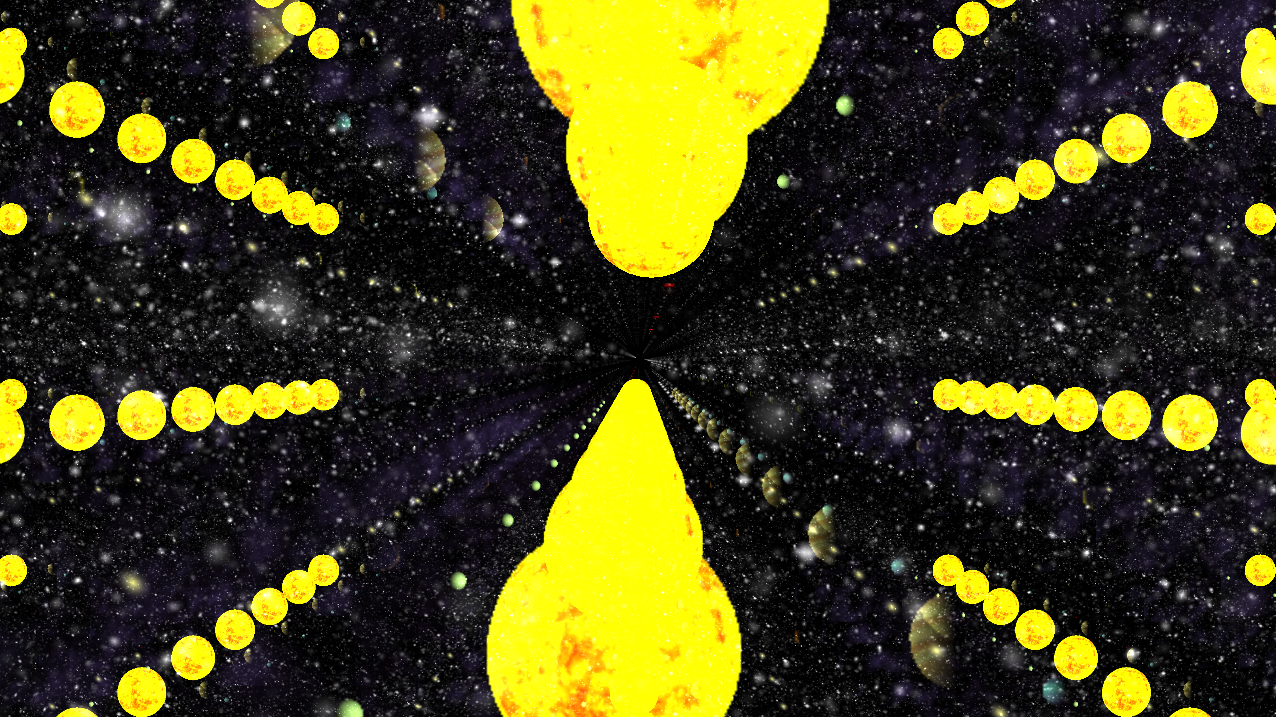
\includegraphics[width=\textwidth]{LensShapes1}
		\caption{Adding 10 ghosts}
	\end{minipage}
	\hfill
	\begin{minipage}[b]{0.4\textwidth}
		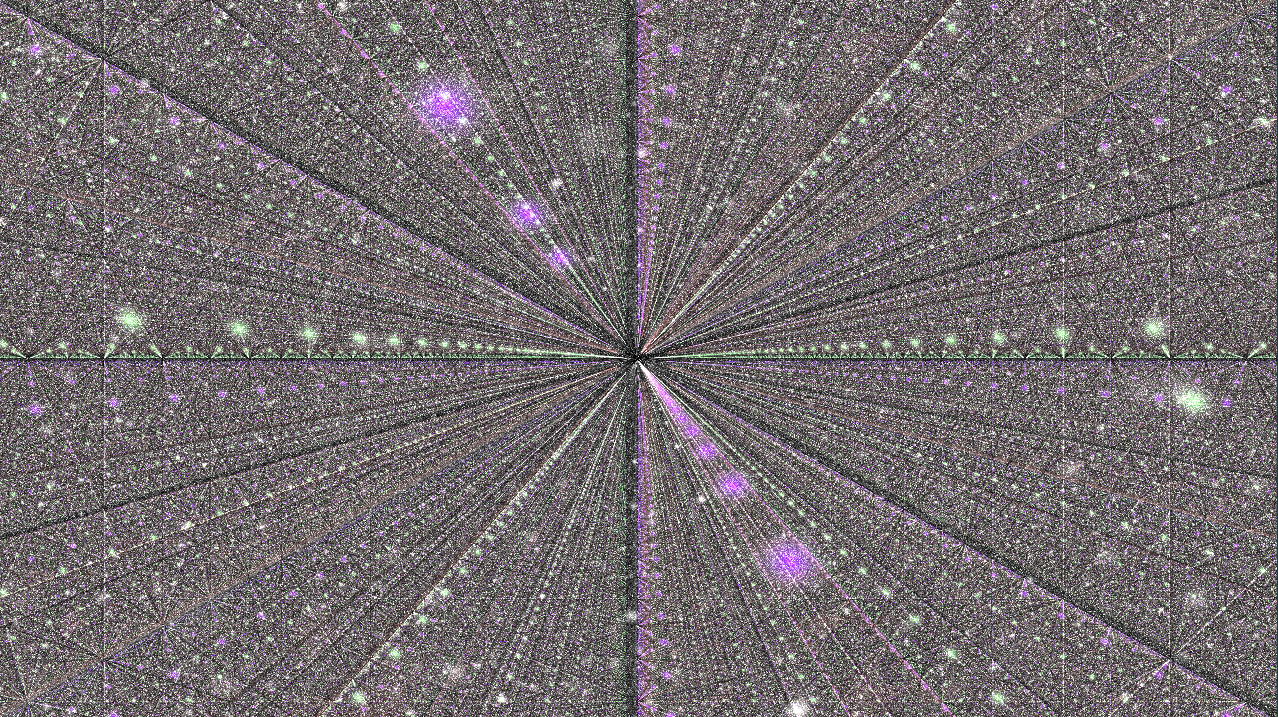
\includegraphics[width=\textwidth]{LensShapes2}
		\caption{Adding 30 ghosts}
	\end{minipage}
\end{figure}
	\fi
\subsection{Multiple Cameras}	
	
		\figuremacro{H}{Project_Falcon}{Millenium Falcon Chase Camera}{ }{1.0}
	
	There are two cameras in this project: a chase camera and a free camera. The free camera allows free movement around the scene, while the chase camera chases around a specific object as it moves, which in our case is the millenium falcon(See figure \textbf{\ref{fig:Project_Falcon}}). This is done by having a global boolean which is set to either true or false every time we want to change the active camera. When we are rendering the objects, we calculate the view matrix using the camera that is currently active. 
	
\subsection{Rotating Planets}	

	The planets rotate around the sun by setting the position of each planet during the update method using cosine for the x axis and sine for the z axis and adding the position of the sun.
	\begin{lstlisting}
	meshes["mercury"].get_transform().position = (vec3(cos(velocity*3.0f)*35.0f, 0.0f, sin(velocity*3.0f)*35.0f) + meshes["sun"].get_transform().position); 
	\end{lstlisting}
	 Velocity is a float. Each time the project goes through the update method, delta time is subtracted from velocity times the equation for an elliptical orbit. The equation applied in this case is not exactly correct, but it results in an approximation of an elliptical orbit for the planets. The x and z of the position is in then multiplied by a number, which is the radius we wish to give to each planet.
	 
\section{Further Work}	 
	
	One of the features I would like to apply in the future is the shadows of all the planets in the plane using a spotlight above the sun. Due to errors, this was not implemented in the scene. Moreover, I would like to apply the correct equation to the velocity of the planets, but I could not completely understand the equation because it required further research, and due to time constraints it was not applied. Finally
	
	
\section{Conclusion}	

	In conclusion, rendering a 3-Dimensional scene using OpenGL and C++ requires a lot of reading around, experimenting, and practising with different visual elements to see what's best. The combination of the variety of techniques being used in this project create an interesting, visually pleasing and gripping result.
	
	


\bibliographystyle{ieeetr}
\bibliography{references}
		
\end{document}
